\documentclass[10pt,a4paper]{article}
\usepackage[margin=1.9cm]{geometry}
\usepackage[T1]{fontenc}
\usepackage{lmodern}
\usepackage{microtype}
\usepackage{amsmath,amssymb}
\usepackage{booktabs,tabularx,array}
\usepackage{xcolor}
\usepackage{listings}
\usepackage{tikz}
\usetikzlibrary{arrows.meta,positioning,shapes.geometric,fit,backgrounds,calc}
\usepackage{pgfplots}
\pgfplotsset{compat=1.18}
\usepackage{enumitem}
\usepackage[hidelinks]{hyperref}
\setlist{nosep,leftmargin=1.4em}
\definecolor{ink}{HTML}{1F2A44}
\definecolor{acc}{HTML}{0F7B6C}
\definecolor{warn}{HTML}{B5462E}
\definecolor{soft}{HTML}{E8F3F1}
\definecolor{softw}{HTML}{F7E9E5}
\lstset{basicstyle=\ttfamily\footnotesize,columns=fullflexible,keepspaces=true,
  frame=single,rulecolor=\color{black!25},backgroundcolor=\color{black!3},
  keywordstyle=\color{ink}\bfseries,language=C,showstringspaces=false}
\tikzset{
  box/.style={draw=ink,rounded corners=3pt,fill=soft,align=center,font=\small,minimum height=9mm,inner sep=4pt},
  dbox/.style={box,fill=softw,draw=warn},
  arr/.style={-{Stealth[length=2.2mm]},thick,draw=ink},
  lab/.style={font=\scriptsize,text=black!70}}
\emergencystretch=1.5em
\usepackage{url}
\def\UrlBreaks{\do\/\do-\do_}
\begin{document}
\thispagestyle{empty}
\vspace*{\fill}
\begin{center}
{\large\scshape\color{ink} Indian Institute of Technology Guwahati}\\[2pt]
{\small\color{black!70} Course Project \quad$\cdot$\quad C-Based VLSI Design (CS5291)}\\[24pt]
{\fontsize{30}{36}\selectfont\bfseries\color{ink} HLSCheck}\\[4pt]
{\large\color{black!70} Approach-1}\\[8pt]
{\Large\itshape\color{acc} Formal equivalence checking of LLM-optimised\\[2pt] HLS code, followed by measured hardware}\\[12pt]
{\color{ink}\rule{0.8\linewidth}{0.6pt}}\\[16pt]
\begin{minipage}[t]{0.48\linewidth}\centering
{\small\scshape\color{acc} Submitted by}\\[4pt]
Dhruvkumar R Pansuriya (230101071)\\
Aryan Kaushik (230101018)\\
Lasya Madhu Sundar (230101058)
\end{minipage}\hfill
\begin{minipage}[t]{0.48\linewidth}\centering
{\small\scshape\color{acc} Instructor}\\[4pt]
Dr.\ Chandan Karfa\\[10pt]
{\small\scshape\color{acc} Date}\\[4pt]
23 November 2026
\end{minipage}\\[16pt]
{\small\color{black!70} Code and saved evidence: \texttt{Project3\_Team.zip}. Every number below comes from our
recorded runs in \texttt{RESULTS.md}.}
\end{center}
\vspace{6pt}
\begin{abstract}
\noindent HLSCheck, our first approach, asks a language model to rewrite a small C kernel so that the hardware made from it is
better, and then answers two separate questions. First, does the rewrite compute exactly the same
thing as the original? Second, if it does, is the hardware actually better? The first question is
answered by a C-to-C equivalence checker that combines our own symbolic executor with the
ESBMC model checker and the Z3 solver. The second is answered by running both versions through the
Bambu HLS tool, simulating the RTL with Verilator, and measuring area with Yosys and timing with
OpenSTA. On our main set of 50 rewrites, all 50 were proved equivalent and all 50 planted faults
were caught; yet only 22 rewrites improved area times latency, 25 made it worse and 3 left it
unchanged. In an 80-case suite of subtle faults, every label matched, and five faults that slipped
past 264 test inputs were still caught by the proof. This report explains how the method works,
which tools it uses, one complete example, and what was measured.
\end{abstract}
\vspace*{\fill}
\newpage

\section{The problem}
Language models are now often asked to ``optimise this kernel for HLS'': unroll a loop, reorder a
loop nest, replace a loop by a bit trick. Two things can go wrong. The rewrite can quietly change what
the function computes, and the rewrite can make the hardware worse even when it is correct.
HLSCheck treats these as two separate decisions and never mixes them:
\begin{enumerate}
\item \textbf{Is it the same function?} For every allowed input, the return value and every final
array element must be equal. This is decided by proof, not by testing alone.
\item \textbf{Is the hardware better?} Only a candidate that passed step 1 is synthesised. Its area,
cycle count and critical-path delay are measured and compared with the original.
\end{enumerate}
A candidate that is not proved equivalent never reaches synthesis, and an ``unknown'' answer is never
counted as ``equivalent''.

\section{The pipeline}
The command \texttt{run\_demo.py original.c candidate.c -{}-function kernel} runs seven stages and saves
the evidence of each one in a fresh run folder.
\begin{center}
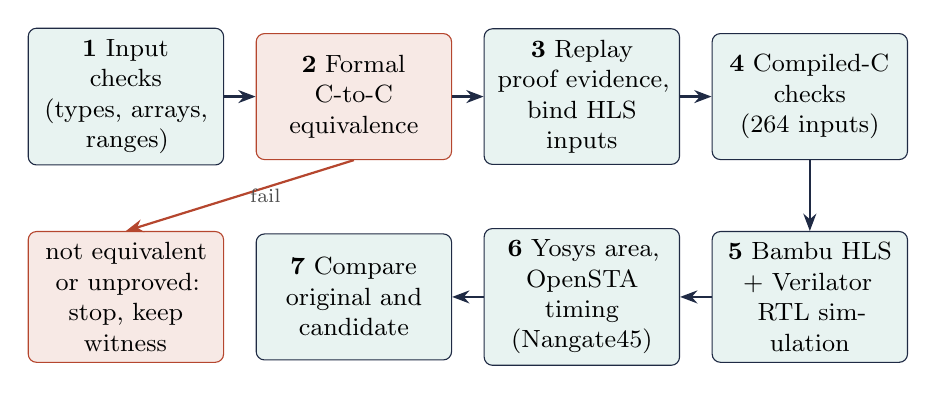
\begin{tikzpicture}[node distance=5mm and 4mm, st/.style={box,text width=22mm,minimum height=16mm}]
\node[st] (s1) {\textbf{1} Input\\checks\\(types, arrays,\\ranges)};
\node[st,right=of s1,fill=softw,draw=warn] (s2) {\textbf{2} Formal\\C-to-C\\equivalence};
\node[st,right=of s2] (s3) {\textbf{3} Replay\\proof evidence,\\bind HLS inputs};
\node[st,right=of s3] (s4) {\textbf{4} Compiled-C\\checks\\(264 inputs)};
\node[st,below=9mm of s4] (s5) {\textbf{5} Bambu HLS\\+ Verilator\\RTL simulation};
\node[st,left=of s5] (s6) {\textbf{6} Yosys area,\\OpenSTA timing\\(Nangate45)};
\node[st,left=of s6] (s7) {\textbf{7} Compare\\original and\\candidate};
\node[dbox,left=of s7,text width=22mm,minimum height=16mm] (stop) {not equivalent\\or unproved:\\stop, keep witness};
\draw[arr] (s1)--(s2); \draw[arr] (s2)--(s3); \draw[arr] (s3)--(s4); \draw[arr] (s4)--(s5);
\draw[arr] (s5)--(s6); \draw[arr] (s6)--(s7);
\draw[arr,draw=warn] (s2.south) -- node[lab,right]{fail} (stop.north);
\end{tikzpicture}
\end{center}
Stage 2 is the heart of the method and is described next. Stage 3 checks the hashes of every proof
file and replays each accepted SMT query, and then makes sure that the exact files proved are the
files given to the HLS tool. Stage 4 compiles both versions and compares them on 264 typed inputs (8
fixed edge patterns and 256 seeded random ones). This is a cross-check, not the proof. Stages 5 to 7
build hardware for both versions with the same settings and report the difference. The exit code is
0 for an equivalent run (even if the hardware got worse), 1 for not equivalent, 2 for unproved and 3
for a pipeline error.

\section{How the equivalence checker works}
\subsection{What ``equivalent'' means here}
Both programs are read through one front end that fixes a target: C11 with ILP32 integer sizes
(\texttt{int} and \texttt{long} are 32 bits, \texttt{long long} is 64). Arrays must be valid and must
not overlap. The observation is the return value and every element of every array parameter at the
end. Both programs must also be free of undefined behaviour (no out-of-bounds access, no signed
overflow, no shift by 32) on every allowed input. Anything outside this model, such as general
pointers, globals, function calls, heap allocation or floating point, is rejected rather than
approximated.

\subsection{The product program}
The usual way to check two programs for equivalence is to glue them into one \emph{product program}:
give both the same symbolic inputs, run one after the other, and assert that the outputs match. A
bounded model checker such as ESBMC then searches for an input that breaks the assertion. This works,
but on kernels with nested loops and multiplications the search can be very slow, because the
checker has to reason about two different loop orders at the same time.

\subsection{Cutting the work with proved regions}
HLSCheck makes the product smaller before ESBMC sees it. The steps are:
\begin{enumerate}
\item \textbf{Pick a boundary.} Find a leading block in each program (declarations and fixed loop
nests) such that no local variable is used after it and no scalar parameter is changed. If no such
block exists, the boundary can be the end of the function.
\item \textbf{Prove the two blocks equal.} Our own symbolic executor unrolls the loops and
builds bit-vector expressions for every array element. Z3 checks that both blocks are safe and leave
equal states for every allowed input.
\item \textbf{Replace both blocks by one shared unknown state.} In the product program, both blocks
are removed and replaced by the same arbitrary array contents. ESBMC then only has to check the rest
of the code (the ``residual''), with all its usual safety checks still on.
\end{enumerate}
\begin{center}
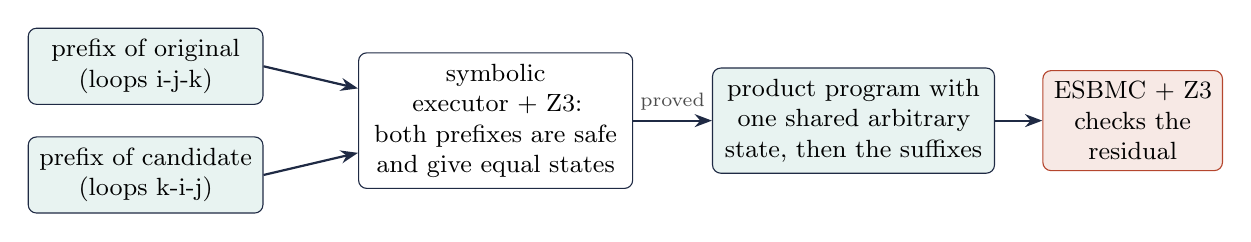
\begin{tikzpicture}[node distance=4mm and 7mm]
\node[box,text width=27mm] (p0) {prefix of original\\(loops i-j-k)};
\node[box,below=of p0,text width=27mm] (p1) {prefix of candidate\\(loops k-i-j)};
\coordinate (m) at ($(p0.east)!0.5!(p1.east)$);
\node[box,right=12mm of m,anchor=west,text width=32mm,fill=white] (z3) {symbolic\\executor + Z3:\\both prefixes are safe\\and give equal states};
\node[box,right=10mm of z3,text width=33mm] (sh) {product program with\\one shared arbitrary\\state, then the suffixes};
\node[box,right=6mm of sh,text width=20mm,fill=softw,draw=warn] (es) {ESBMC + Z3\\checks the\\residual};
\draw[arr] (p0.east) -- (z3); \draw[arr] (p1.east) -- (z3);
\draw[arr] (z3) -- node[lab,above]{proved} (sh); \draw[arr] (sh) -- (es);
\end{tikzpicture}
\end{center}
\textbf{Why this is sound.} Call the prefixes $P_0,P_1$ and the suffixes $S_0,S_1$. Step 2 proves
that for every input $I$, $P_0(I)$ and $P_1(I)$ are safe and leave the same state. So every real
pair of prefix results is one of the ``equal arbitrary states'' used in step 3. If the suffixes agree
for \emph{all} equal states, they agree for the real ones too.

\subsection{When the shortcut loses information: refinement}
The reverse is not true. A shared arbitrary state forgets how the arrays were computed, so ESBMC may
report a mismatch that cannot really happen. A typical case is a suffix that returns \texttt{out[i]}
in one program and \texttt{13*a[i]} in the other: the two are equal only because the prefix set
\texttt{out[i] = 13*a[i]}, and the shared state has lost that fact. HLSCheck handles this in a loop:
\begin{center}
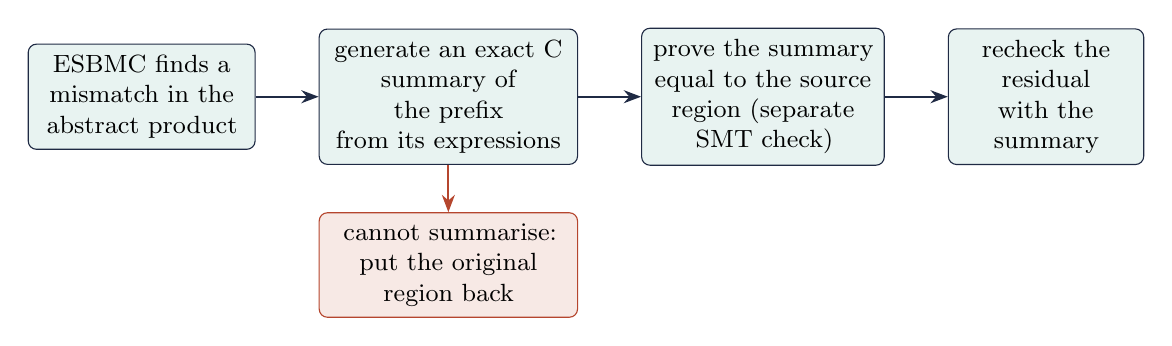
\begin{tikzpicture}[node distance=5mm and 8mm]
\node[box,text width=26mm] (r) {ESBMC finds a\\mismatch in the\\abstract product};
\node[box,right=of r,text width=30mm] (g) {generate an exact C\\summary of the prefix\\from its expressions};
\node[box,right=of g,text width=28mm] (c) {prove the summary\\equal to the source\\region (separate SMT check)};
\node[box,right=of c,text width=22mm] (rc) {recheck the\\residual with the\\summary};
\node[dbox,below=6mm of g,text width=30mm] (orig) {cannot summarise:\\put the original\\region back};
\draw[arr] (r)--(g); \draw[arr] (g)--node[lab,above]{}(c); \draw[arr] (c)--(rc);
\draw[arr,draw=warn] (g)--(orig);
\end{tikzpicture}
\end{center}
The summary generator is not trusted: its output is itself proved equal to the code it replaces.
If no summary can be made, the original code goes back into the product, which is just the plain
product program again. With the summary in place, the \texttt{13*a[i]} example is proved equal,
while a candidate returning \texttt{13*a[i]+1} still fails with a real input.

\subsection{Checking counterexamples}
When the whole-function symbolic check finds a mismatch, it proposes a concrete input. ESBMC then
checks the real, unabstracted pair at that input. Only a confirmed mismatch counts as ``not
equivalent''. If the two programs agree at that input, the proposal is thrown away and the full
input domain is checked instead, because agreement at one input proves nothing. Every confirmed
mismatch is also compiled and run natively, and the native outputs must match the solver's.

\subsection{What a verdict contains}
Each run returns one of equivalent, not equivalent, candidate undefined, unsupported or inconclusive,
together with the contract, the region lemmas, the summary lemmas, the refinement history, the
residual proof, all accepted SMT queries (exported so they can be replayed) and the concrete input
if there is one. The limit is 60 seconds per solver call; incomplete loop unwinding gives
inconclusive, never equivalent.

\section{One complete run: matrix multiply with a different loop order}
The project includes two 4$\times$4 matrix multiply files. \texttt{matmul.cpp} uses the loop order
i-j-k, and \texttt{matmul\_opti.cpp} uses k-i-j. Both zero the output and add
\texttt{a[i*4+k]*b[k*4+j]} into \texttt{out[i*4+j]}, with unsigned 32-bit wrap-around.
\begin{lstlisting}
/* original: i-j-k */                       /* candidate: k-i-j */
for (i = 0; i < 4; i++)                     for (k = 0; k < 4; k++)
  for (j = 0; j < 4; j++)                     for (i = 0; i < 4; i++)
    for (k = 0; k < 4; k++)                     for (j = 0; j < 4; j++)
      out[i*4+j] += a[i*4+k] * b[k*4+j];          out[i*4+j] += a[i*4+k] * b[k*4+j];
\end{lstlisting}
This is the console output of our saved run (a few progress lines removed):
\begin{lstlisting}[language={}]
[2/7] FORMAL C-TO-C EQUIVALENCE
  region_equality: equivalent [custom symbolic execution / Z3]
  residual_0: equivalent [ESBMC / Z3]
  VERDICT: equivalent (0.532 s)
[3/7] REPLAY PROOF EVIDENCE AND BIND HLS INPUTS
  Proof artifact hashes: PASS; accepted SMT queries replayed: 1.
[4/7] COMPILED-C EDGE/RANDOM CHECKS
  PASS: 264 typed edge/random comparisons
[5/7] HLS GENERATION AND RTL SIMULATION
  [original] RTL simulation: PASS, 16 transactions, 266 average cycles
  [optimized] RTL simulation: PASS, 16 transactions, 314 average cycles
[6/7] CELL MAPPING AND STATIC TIMING (per design)
  [original] Mapped area: 4612.972 um^2
  [optimized] Mapped area: 5004.258 um^2
  [original] Critical-path delay: 1.865742 ns; meets 10 ns: True
  [optimized] Critical-path delay: 1.834684 ns; meets 10 ns: True
[7/7] MEASURED QUALITY COMPARISON
  Latency speedup: 0.847x
  Area x latency outcome: REGRESSED
\end{lstlisting}
The proof took half a second: the loop nests were proved equal as one region, and the empty residual
was then checked by ESBMC. The ``optimised'' version is correct but worse:
\begin{center}\small
\begin{tabular}{@{}lrrr@{}}\toprule
metric & original & candidate & improvement\\\midrule
area ($\mu$m$^2$) & 4612.97 & 5004.26 & $-8.48\%$\\
latency (cycles) & 266 & 314 & $-18.05\%$\\
critical-path delay (ns) & 1.866 & 1.835 & $+1.66\%$\\
area $\times$ latency & $1.227\times10^7$ & $1.571\times10^7$ & $-28.06\%$\\\bottomrule
\end{tabular}
\end{center}
Improvement is $100\times(\text{original}-\text{candidate})/\text{original}$, so a positive number is
better. The file \texttt{matmul\_wrong.cpp} changes one multiplication into an addition; the checker
reports a concrete input where the outputs differ, replays it natively, and stops before HLS.

\section{Tools}
\begin{center}\small
\noindent\begin{tabularx}{\linewidth}{@{}>{\raggedright\arraybackslash}p{3.1cm}X@{}}\toprule
tool & what it does in HLSCheck\\\midrule
own symbolic executor & written by us; unrolls supported loops and builds bit-vector expressions for region proofs and summaries\\
Z3 & SMT solver; proves region equality and summary correctness; also ESBMC's back end\\
ESBMC & bounded model checker for C, used unmodified; checks the residual product program with bounds, pointer, overflow, division, shift, uninitialised and unwinding checks\\
Clang & compiles both versions for the 264-input native comparison and for witness replay\\
Bambu 2026.11 & open-source HLS tool; C to Verilog (BAMBU-BALANCED-MP, -O2, seed 0)\\
Verilator & simulates the generated RTL (16 transactions per design in the demo)\\
Yosys 0.36 + Nangate45 & maps the design to standard cells and reports area in $\mu$m$^2$\\
OpenSTA 2.0.18 & static timing at a common 10 ns clock; reports the critical path\\
Qwen2.5-Coder-1.5B, GPT-6.1-Sol & the models that wrote candidates (Qwen locally, GPT through Codex tasks); no paid API\\\bottomrule
\end{tabularx}
\end{center}
Hardware numbers are pre-layout ASIC estimates, not FPGA resource counts or routed timing. RTL
simulation is a sampled check, not a proof that the RTL matches the C.

\section{How it was tested}
We built several groups of test cases. They overlap (some pairs are rechecked in later
studies), so the counts should not be added up.
\begin{center}\small
\noindent\begin{tabularx}{\linewidth}{@{}>{\raggedright\arraybackslash}p{2.8cm}X>{\raggedright\arraybackslash}p{4.2cm}@{}}\toprule
group & how the cases were made & checks run\\\midrule
Main cohort & 50 original/rewrite pairs (47 distinct originals) written with LLM help: reductions,
bit tricks, filters, images, linear algebra, data movement; plus one planted fault per pair & proof,
13{,}200 native trials, 50 witness replays, 100 hardware builds, 1{,}600 RTL transactions\\
Two-model study & 12 inputs from MachSuite, CHStone and HLS-Eval; one first answer per model, no
repair & proof, 34 hardware builds, 544 RTL transactions\\
Local-model run & 20 kernels $\times$ 2 seed/temperature settings, Qwen 1.5B, raw first answers & proof;
hardware for the 9 changed equivalent answers\\
Subtle faults & 50 small edits (index, bound, mask, coefficient), 4 semantic traps, 20 equivalent
edits, 6 undefined-C cases; labels fixed before running & proof, native witness replay\\
Integrated checker & 239 rechecks of cases from all groups above with the final checker & label
agreement, SMT replay\\
Larger instances & 27 scaled pairs (e.g.\ 16$\times$16 GEMM, 128-element prefix) & proof only\\
Public leaves, EqBench & 8 real leaf functions from CHStone, MachSuite, HLS-Eval (+8 planted bugs);
14 eligible EqBench pairs & proof, 96{,}272 native trials\\\bottomrule
\end{tabularx}
\end{center}

\section{Results}
\subsection{Correctness}
\begin{center}\small
\begin{tabular}{@{}lrl@{}}\toprule
group & cases & outcome\\\midrule
Main cohort rewrites & 50 & all 50 proved equivalent\\
Main cohort planted faults & 50 & all 50 rejected with a witness\\
Subtle faults & 80 & 80 of 80 labels match (54 rejected, 20 accepted, 6 undefined)\\
Integrated checker & 239 & 236 of 237 known labels match; 1 known-equivalent case inconclusive\\
Local Qwen answers & 40 & 28 equivalent, 8 not equivalent, 2 undefined, 1 unsupported, 1 unknown\\
Two-model study, Qwen & 12 & 12 equivalent (9 of them unchanged code)\\
Two-model study, GPT & 12 & 10 equivalent, 2 inconclusive (ATAX, BiCG)\\
Public leaves & 16 & 8 rewrites equivalent, 8 planted bugs rejected\\
EqBench & 14 & 2 equivalent (both match), 9 incomplete unwind, 3 unknown\\
Larger instances & 29 & 22 equivalent, 3 not equivalent, 4 inconclusive\\\bottomrule
\end{tabular}
\end{center}
In the integrated study, summaries were used in 120 cases and refinement was needed in 22. All
accepted SMT queries replayed, and all 121 concrete mismatch inputs reproduced a difference in
compiled C. The eight wrong answers from the local model were real mistakes: wrong FIR coefficients,
XOR used as absolute difference, broken prefix logic, wrong SYRK indexing, overlapping popcount
groups, bad bit-reversal shifts, a spurious zero-input special case and a convolution offset.

\textbf{Proof beats testing on rare faults.} Five subtle faults passed all 264 native test inputs but
were caught by the proof, with the witness confirmed natively: \texttt{all\_equal16} (differences
cancel under XOR), \texttt{clamp16} (clamp one bit too early), \texttt{threshold\_pack8} (a rare
equality boundary), \texttt{search\_count16} (wrong lane) and \texttt{fault\_rare\_magic}.

\subsection{Hardware}
Of the 50 proved-equivalent rewrites in the main cohort, area times latency (ALP) improved for 22,
got worse for 25 and was unchanged for 3. Area improved in 14 pairs, cycles in 34 and critical-path
delay in 11. All 100 designs met the 10 ns clock. The chart shows the ALP change of every pair,
sorted.
\begin{center}
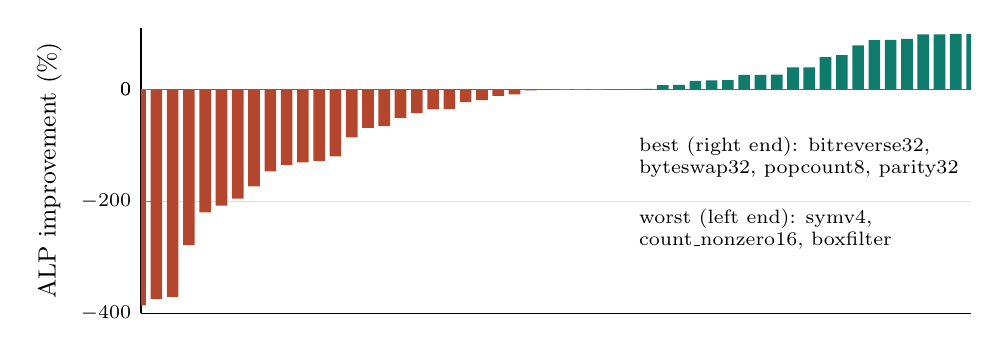
\begin{tikzpicture}
\begin{axis}[width=\linewidth,height=5.2cm,ybar,bar width=4.2pt,ymin=-400,ymax=110,xmin=0,xmax=51,
  xtick=\empty,ylabel={ALP improvement (\%)},ylabel style={font=\small},tick label style={font=\scriptsize},
  ymajorgrids,grid style={black!12},axis lines*=left,
  extra y ticks={0},extra y tick style={grid style={black!60}}]
\addplot[fill=warn,draw=none] coordinates {(1,-386.03) (2,-374.99) (3,-370.87) (4,-278.26) (5,-219.74) (6,-207.66) (7,-195.15) (8,-172.98) (9,-146.42) (10,-134.62) (11,-130.30) (12,-127.45) (13,-119.36) (14,-85.30) (15,-68.54) (16,-65.46) (17,-50.48) (18,-42.07) (19,-35.38) (20,-34.89) (21,-22.42) (22,-18.63) (23,-11.04) (24,-8.61) (25,-1.29)};
\addplot[fill=black!35,draw=none] coordinates {(26,0.4) (27,0.4) (28,0.4)};
\addplot[fill=acc,draw=none] coordinates {(29,0.27) (30,1.34) (31,8.02) (32,8.38) (33,15.85) (34,16.86) (35,17.13) (36,26.35) (37,26.42) (38,26.96) (39,39.73) (40,40.14) (41,58.25) (42,61.66) (43,79.38) (44,88.75) (45,88.96) (46,91.04) (47,98.87) (48,99.11) (49,99.97) (50,100.00)};
\node[font=\scriptsize,anchor=west,align=left] at (axis cs:30,-250) {worst (left end): symv4,\\count\_nonzero16, boxfilter};
\node[font=\scriptsize,anchor=west,align=left] at (axis cs:30,-120) {best (right end): bitreverse32,\\byteswap32, popcount8, parity32};
\end{axis}
\end{tikzpicture}
\end{center}
The wins come from real algorithmic changes: prefix reuse (62 to 26 cycles, about half the area,
$+79.4\%$ ALP), XOR-fold parity (34 cycles to 1, $+98.9\%$), byte-parallel popcount ($+99.1\%$).
The losses come mostly from unrolling: fewer cycles but much more area, for example \texttt{sum32}
(35 to 19 cycles but almost 7 times the area, $-278\%$ ALP). A pair counts as improved only if ALP drops by at least 0.1\%; the three grey
bars are the unchanged pairs.

\textbf{Two models.} On 10 inputs where both models' answers were measured, GPT-6.1-Sol had a
geometric-mean latency speedup of 1.258$\times$ and an ALP ratio of 0.972; Qwen 1.5B had 0.937$\times$ and
1.066. GPT's SYRK rewrite was the clear win (232 to 100 cycles, $+74\%$ ALP), while its GEMM, stencil
and MVT rewrites were faster but larger overall. Nine of Qwen's twelve answers were the original code
unchanged, which shows that ``equivalent'' does not mean ``optimised''.

\subsection{Time}
The limit is 60 seconds per solver call, not per pair. Some measured proof times: 4$\times$4 matmul in
0.53 s, 16$\times$16 GEMM in 3.4 s, indexed 16$\times$16 GEMM in 15.8 s, 128-element prefix in 2.6 s,
128-element dot product in 0.96 s, 64-tap FIR in 0.71 s and 16$\times$16 stencil in 2.5 s. On one
targeted case the combined method proved an indexed GEMM in 1.06 s where plain ESBMC hit its limit;
on another, plain ESBMC found a wrong-array bug faster (0.56 s against 2.65 s).

\section{A second check with VWE}
We later built a second tool, VWE (Approach-2, described in its own report), and ran it on 181 of HLSCheck's cases: the main
cohort's 51 equivalent and 50 not-equivalent pairs and the 80 subtle-fault controls. VWE treats each
pair as the request ``optimise without changing behaviour'' and uses CBMC instead of ESBMC. It
decided 125 cases and agreed with HLSCheck's label on all 125, including the five test-escaping
faults. It left 56 undecided, mostly because it could not certify a safe reference region within its
bounds. Two different tools reaching the same answers adds confidence in those labels.

\section{Strengths and limits}
\textbf{Strengths.} Correctness and hardware benefit are kept apart, so a correct but slower rewrite
is reported as exactly that. Every positive answer is backed by replayable SMT queries and every
negative one by a natively reproduced input. Unknown stays unknown. The planted faults and the 20
``equivalent but changed'' controls test both directions.

\textbf{Limits.} The front end accepts only integer kernels with fixed-size, non-overlapping arrays;
pointers, globals, calls and floating point are out. Only one region (a prefix or the whole function)
is abstracted, and loop invariants are not inferred, so loops that depend on inputs can stay
inconclusive. Hardware numbers are pre-layout estimates for one ASIC library, not FPGA results. The
test cases are related educational kernels, so the 22/25/3 split describes these cases, not LLMs in
general.

\section{Conclusion}
HLSCheck gives a complete and careful path from an LLM's rewrite to a measured hardware result,
with a proof gate in the middle. Its checker caught every planted and subtle fault in its own
suites, including faults that tests missed, and its use of proved regions makes the remaining
model-checking problem smaller. The hardware results are the most useful lesson: half of the
proved-correct ``optimisations'' made the hardware worse. Equivalence checking tells you a rewrite is
safe to use; only measurement tells you whether it is worth using.

\section*{References}
\begin{enumerate}[label={[\arabic*]},leftmargin=2em]
\item HLSCheck code and saved evidence, \texttt{Project3\_Team.zip}: the README, the results
overview, the algorithm and pipeline notes, and the subtle-fault report.
\item M. R. Gadelha, F. R. Monteiro, J. Morse, L. C. Cordeiro, B. Fischer, D. A. Nicole. ESBMC 5.0: an
industrial-strength C model checker. In \emph{ASE}, 2018.\newline\url{https://github.com/esbmc/esbmc}
\item L. de Moura, N. Bj{\o}rner. Z3: an efficient SMT solver. In \emph{TACAS}, LNCS 4963, Springer, 2008.
\item F. Ferrandi et al. Bambu: an open-source research framework for the high-level synthesis of
complex applications. In \emph{DAC}, 2021. \url{https://github.com/ferrandi/PandA-bambu}
\item W. Snyder. Verilator. \url{https://www.veripool.org/verilator/}
\item C. Wolf. Yosys Open SYnthesis Suite. \url{https://yosyshq.net/yosys/}
\item OpenSTA static timing analyser. \url{https://github.com/The-OpenROAD-Project/OpenSTA}
\item B. Reagen, R. Adolf, Y. S. Shao, G.-Y. Wei, D. Brooks. MachSuite: benchmarks for accelerator
design and customized architectures. In \emph{IISWC}, 2014.
\item Y. Hara, H. Tomiyama, S. Honda, H. Takada. Proposal and quantitative analysis of the CHStone
benchmark program suite for practical C-based high-level synthesis. \emph{J. Information Processing}, 2009.
\item A. Pnueli, M. Siegel, E. Singerman. Translation validation. In \emph{TACAS}, 1998.
\item G. Barthe, J. M. Crespo, C. Kunz. Relational verification using product programs. In \emph{FM}, 2011.
\end{enumerate}
\end{document}
